\subsection{Tabu Search} \label{subsec:Grundlagen_TabuSearch}

Die Tabu Search (zu dt. Tabu-Suche) wurde von Fred Glover im Jahre 1986 vorgeschlagen \cite[vgl.][S. 37]{gendreau_handbook_2019} und gilt als eine Erweiterung der \acf{LS}, welche bereits im übergeordneten Abschnitt eingeführt wurde. Der Vorteil der \acf{TS} gegenüber der \ac{LS} ist der Umgang mit lokalen Optima über das Nutzen einer Tabu-Liste. Hierbei werden Lösungen innerhalb einer Nachbarschaft ausgeschlossen, die sich bereits in der Tabu-Liste befinden. Die lokale Suche samt Einhaltung einer Tabu-Liste als Kurzzeitgedächtnis stellt die Basisversion der \ac{TS} dar. \cite[vgl.][S. 40]{gendreau_handbook_2019} \\

Beim Erreichen eines lokalen Optimums findet innerhalb der \ac{LS} in jeder Iteration ein repetitiver Wechsel zweier Lösungen statt. Durch diese Wechselschleife bis zur Terminierung des Algorithmus wird das lokale Optimum nicht mehr verlassen. \cite[vgl.][S. 40]{gendreau_handbook_2019} 

\begin{lstlisting}[caption={Tabu Search (Quelle: \cite[vgl.][S. 42 ff.]{gendreau_handbook_2019}}), label=lst:tabusearch, mathescape=truexinputencoding={utf8}, extendedchars=false, escapeinside=``]
Create an initial solution $s$ inside the search space;
Init tabu list $TL \leftarrow \emptyset$;
while stopping criteria not satisfied do
    Select best solution $s' \in N(s) \setminus TL$;
    $s \leftarrow s'$; 
    Add $s'$ to the tabu list $TL$;
    If tabu list $TL$ is full, remove oldest entry;
end
return the best solution;
\end{lstlisting}

Listing \ref{lst:tabusearch} beschreibt den Algorithmus der Tabu-Suche. Eine Tabu-Liste $TS$ stellt das Kurzzeitgedächtnis dar, welches nur eine feste Anzahl an Einträgen beinhalten kann und im initialen Zustand zunächst leer ist. Die Größe der Tabu-Liste $|TS]$ stellt ein Hyperparameter dar, welcher somit bei der Implementierung zu definieren ist. In jeder Iteration wird die ausgewählte Lösung, welche der besten Lösung einer Nachbarschaft entspricht, in die Tabu-Liste an erster Stelle hinzugefügt. Bestehende Einträge werden folglich um eine Stelle in der Liste weiterpropagiert. Einträge aus der Tabu-Liste dürfen nicht mehr aus einer Nachbarschaft $N(s)$ ausgewählt werden. Sofern die Tabu-Liste voll ist, wird das älteste Element entfernt und darf somit wieder ausgewählt werden. Durch das Ausschließen der Listeneinträge ist ein repetitiver Wechsel zweier Lösungen, wie es bei der \ac{LS} der Fall ist, je nach Größe der Tabu-Liste vermeidbar. Zudem wird der Suchraum um einen größeren Bereich erkundet und lokale Optima können verlassen werden. \cite[vgl.][S. 42 ff.]{gendreau_handbook_2019} \\

Sowohl in der lokalen Suche als auch in der Tabu-Suche ist eine Nachbarschaftsfunktion vorgesehen. Die Nachbarschaftsfunktion $N(s)$ stellt eine Submenge von Lösungen eines Suchraums dar. Diese beinhaltet Lösungen, welche von einer Ausgangslösung $s$ mit einem Move $m$ (dt. Schritt) erreichbar sind. Ein Move $m$ wird als eine charakterisierte Modifikation an einer Lösung bezeichnet. \cite[vgl.][S. 56]{siarry_metaheuristics_2016} \\

Beispielhaft visualisiert Abbildung \ref{img:example_neighbourhood} den Lösungsraum einschließlich der Nachbarschaftsbeziehungen von allen Permutationen von vier Elementen. Die Nachbarschaftsbeziehungen unterscheiden sich je nach Optimierungsproblem und müssen folglich für jedes Problem gesondert selektiert werden \cite[vgl.][S. 57 f.]{siarry_metaheuristics_2016}. Gemäß des Beispiels in der Abbildung wäre die Nachbarschaft für die Lösung 1234 über $N(1234) = \{ 1324, 1432, 2134 \}$ definiert, da nur ein Move notwendig ist, um diese Lösungen zu erreichen.  

\begin{figure}[H]
    \centering
    \noindent\makebox[\textwidth]{%
    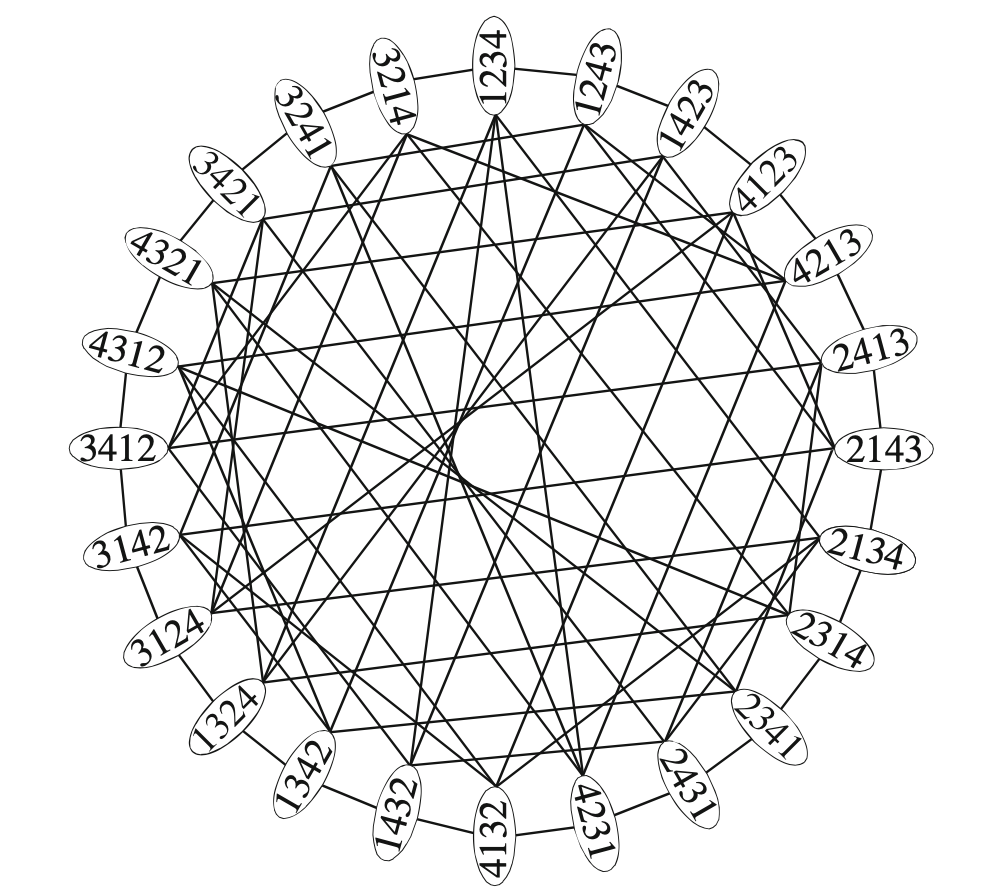
\includegraphics[width=0.74\textwidth]{assets/img/02_Grundlagen/Neighbourhood.png}
    }
    \caption{Nachbarschaftsbeziehungen einer Menge von Permutationen aus vier Elementen in Knotenform} 
    \label{img:example_neighbourhood}
    \source{\cite[][S. 57]{siarry_metaheuristics_2016} }
\end{figure}

Bei der Tabu-Suche stehen wie auch bei anderen Metaheuristiken, unterschiedliche Möglichkeiten zur Terminierung der Algorithmen zur Verfügung. Ein Algorithmus kann nach einer festen Anzahl an Iterationen oder CPU-Zeit beendet werden. Ein Algorithmus kann zudem auch nach einer bestimmten Anzahl an Iterationen, wo keine Verbesserung der Zielfunktion vorzufinden ist, terminiert werden. Eine weitere Möglichkeit ist, dass ein Algorithmus solange durchiteriert wird, bis ein definierter Schwellwert erreicht wurde. \cite[vgl.][S. 44]{gendreau_handbook_2019} 
